\section{Experiments}
\subsection{Experimental Setup}
\label{sec:exp_setup}

\paragraph{Models and Datasets} 
We primarily evaluate our method using LLaMA-3.1-8B-Instruct~\cite{dubey:2024llama3} and Qwen2.5-Instruct series~\cite{Qwen2}. The evaluation leverages two widely-used math reasoning benchmarks: GSM8K~\citep{Cobbe:2021gsm8k} and MATH~\cite{math}. For training, we use the respective training sets from both datasets. Regarding the MATH dataset, due to the computation cost, we assess our method on a subset, MATH-500, which is identical to the test set used in \citet{Lightman:2024verify}.

\paragraph{Implementation Details} 
We utilize LLMLingua-2~\cite{pan:2024llmlingua2} as the token importance metric to generate our compressed CoT training data. The compression ratio $\gamma$ is randomly selected from the ratio set $\{0.5, 0.6, 0.7, 0.8, 0.9, 1.0\}$ for each training sample. We adopt LoRA~\cite{lora} to train our models. \method is characterized by its low training cost, with training taking $\sim$2 hours for the 7B model and $\sim$2.5 hours for the 14B model on 3090 GPUs. We include more implementation details in Appendix~\ref{appendix:training_details}.

\paragraph{Baselines} 
We compare \method to three baselines: \textbf{1) Token-efficient Prompts.} Following \citet{Lee:2025Complexity}, we select three advanced prompts, instructing LLMs to perform CoT efficiently. These prompts, denoted as \texttt{BeConcise}, \texttt{OnlyNumbers}, and \texttt{AbbreWords}, are detailed in Appendix~\ref{appendix:prompt_detail}; \textbf{2) Length-control Prompts.} We instruct the LLM to reduce a fixed proportion of output tokens in the CoT process, denoted as \texttt{LC-Prompt} in Table~\ref{tab:main}; \textbf{3) Truncation.} This method involves brute-force length truncation, where the maximum number of output tokens is restricted, compressing the CoT output to a fixed ratio.

\begin{figure}[t]
\centering
    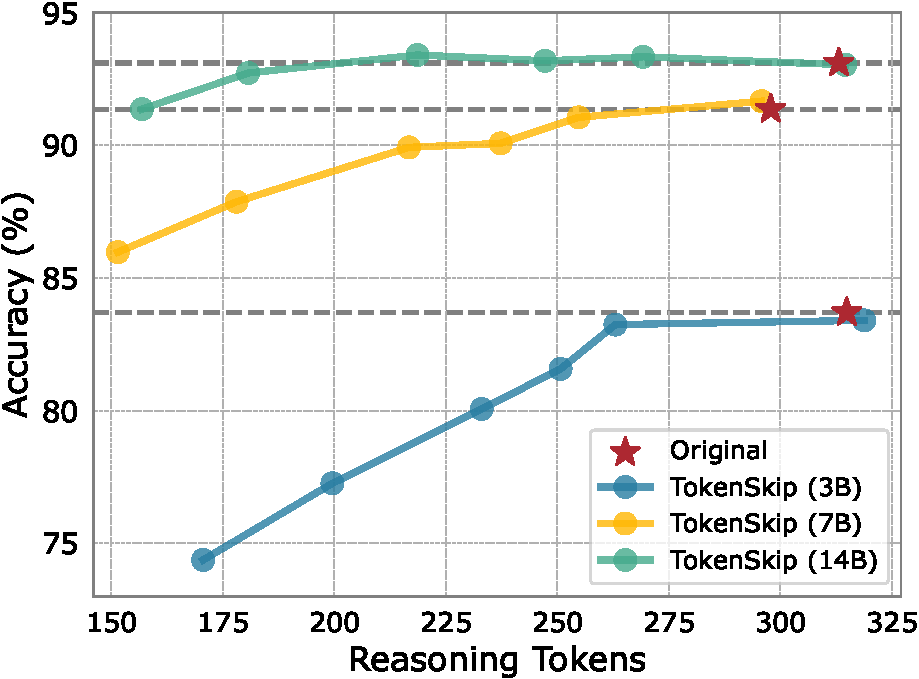
\includegraphics[width=0.95\columnwidth]{fig/scaling.pdf}
    \caption{Compression performance of \method on Qwen2.5-Instruct models. Qwen2.5-14B-Instruct shows almost \textbf{no} performance drop with $\bm{40\%}$ token trimming.}
    \label{fig:qwen-scaling}
\end{figure}

\paragraph{Evaluation Metrics} 
We evaluate \method using three widely used metrics: accuracy, the number of CoT tokens, and inference latency per sample. Model performance is assessed using scripts from \texttt{DeepSeek-Math}\footnote{\url{https://github.com/deepseek-ai/DeepSeek-Math}}. Greedy decoding is employed to generate the outputs from the target LLM. Inference latency is measured on a single NVIDIA 3090 GPU with a batch size of 1. In addition to these metrics, we report the actual compression ratio of the CoTs to assess whether the compression aligns with the specified ratio.

\begin{table*}[t]
\centering
\small
\setlength{\tabcolsep}{1.4mm}
\begin{tabular}{@{}lcrrrcrrrc@{}}
\toprule
\multirow{2}{*}{\textbf{Methods}} &\multirow{2}{*}{$\textbf{Ratio}$} & \multicolumn{4}{c}{\textbf{GSM8K}}  & \multicolumn{4}{c}{\textbf{MATH-500}} \\ \cmidrule(lr){3-6} \cmidrule(lr){7-10}
&  &Accuracy $\uparrow$ &Tokens $\downarrow$ &Latency (s) $\downarrow$ &\textit{Act}Ratio   &Accuracy $\uparrow$ &Tokens $\downarrow$ &Latency (s) $\downarrow$ &\textit{Act}Ratio  \\ \midrule
\texttt{Original}  & - & 86.2\cred{(0.0 \downarrow)} &213.17 &5.96\cred{1.0\times} &-  & 48.6\cred{(0.0 \downarrow)} & 502.60  &16.37\cred{1.0\times} &- \\ \midrule
\texttt{BeConcise}  & - & 82.9\cred{(3.3 \downarrow)} &161.32 &4.73\cred{1.3\times} &0.76  & 47.4\cred{(1.2 \downarrow)} & 471.34  &15.54\cred{1.1\times} &0.94 \\
\texttt{OnlyNumbers}  & - & 83.2\cred{(3.0 \downarrow)} &165.27 &4.95\cred{1.2\times} &0.78  & 46.4\cred{(2.2 \downarrow)} & 487.00  &15.93\cred{1.0\times} &0.97 \\
\texttt{AbbreWords}  & - & 83.7\cred{(2.5 \downarrow)} &170.33 &5.15\cred{1.2\times} &0.80  & 47.6\cred{(1.0 \downarrow)} & 489.07  &15.94\cred{1.0\times} &0.97 \\ \midrule
\multirow{3}{*}{\texttt{LC-Prompt}}  &0.9 & 84.1\cred{(2.1 \downarrow)} &226.37 &6.12\cred{1.0\times} & 1.06  & 48.6\cred{(0.0 \downarrow)} &468.04 &15.39\cred{1.1\times} & 0.93  \\
&0.7 & 84.9\cred{(1.3 \downarrow)} &209.39 &5.51\cred{1.1\times} & 0.98  & 48.4\cred{(0.4 \downarrow)} &472.13 &15.55\cred{1.1\times} & 0.94  \\
&0.5 & 83.7\cred{(2.5 \downarrow)} &188.82 &4.97\cred{1.2\times} & 0.89  & 47.8\cred{(0.4 \downarrow)} &471.11 &15.48\cred{1.1\times} & 0.94  \\ \midrule
\multirow{3}{*}{\texttt{Truncation}}  &0.9 & 70.2\cred{(26.0 \downarrow)} &202.06 &5.29\cred{1.1\times} & 0.95  & 47.8\cred{(0.8 \downarrow)} &440.33 &14.56\cred{1.1\times} & 0.88  \\
&0.7 & 25.9\cred{(60.3 \downarrow)} &149.99 &3.97\cred{1.5\times} & 0.70  & 45.0\cred{(3.6 \downarrow)} &386.89 &12.85\cred{1.3\times} & 0.77  \\
&0.5 & 7.0\cred{(79.2 \downarrow)} &103.69 &2.95\cred{2.0\times} & 0.49  & 27.4\cred{(21.2 \downarrow)} &283.70 &9.40\cred{1.7\times} & 0.56  \\ \midrule
\multirow{6}{*}{\method}  &1.0 & 86.7\cred{(0.5 \uparrow)} &213.60 &5.98\cred{1.0\times} & 1.00  & 48.2\cred{(0.4 \downarrow)} &504.79 &16.43\cred{1.0\times} & 1.00  \\
&0.9 & 86.1\cred{(0.1 \downarrow)} &198.01 &5.65\cred{1.1\times} & 0.93  & 47.8\cred{(0.8 \downarrow)} & 448.31  & 15.26\cred{1.1\times} & 0.89 \\
&0.8 & 84.3\cred{(1.9 \downarrow)} &169.89 &5.13\cred{1.2\times} & 0.80  & 47.3\cred{(1.3 \downarrow)} & 398.94  & 13.39\cred{1.2\times} & 0.79 \\
&0.7 & 82.5\cred{(3.7 \downarrow)} &150.12 &4.36\cred{1.4\times} & 0.70  & 46.7\cred{(1.9 \downarrow)} & 349.13  & 11.55\cred{1.4\times} & 0.69 \\
&0.6 & 81.1\cred{(5.1 \downarrow)} &129.38 &3.81\cred{1.6\times} & 0.61  & 42.0\cred{(6.6 \downarrow)} & 318.36  & 10.58\cred{1.6\times} & 0.63 \\
&0.5 & 78.2\cred{(8.0 \downarrow)} &113.05 &3.40\cred{1.8\times} & 0.53  & 40.2\cred{(8.4 \downarrow)} & 292.17  & 9.67\cred{1.7\times} & 0.58 \\
\bottomrule
\end{tabular}
\caption{Experimental results of \method on LLaMA-3.1-8B-Instruct. We report accuracy, average CoT token count (Tokens), average latency per sample, and actual compression ratio (\textit{Act}Ratio) for comparison.}
\label{tab:main}
\end{table*}

\subsection{Main Results}
\label{sec:main-exp}
The performance of \method on GSM8K using the Qwen2.5-Instruct series\footnote{For detailed results, please refer to Appendix~\ref{appendix:qwen_detail}.} is illustrated in Figure~\ref{fig:qwen-scaling}. As the model scale increases, there is less performance degradation at higher compression ratios, indicating that larger LLMs are better at identifying shortcuts between critical reasoning tokens, enabling more efficient CoT generation. Notably, Qwen2.5-14B-Instruct exhibits almost \textbf{NO} performance drop (less than $0.4\%$) with $\bm{40\%}$ token trimming. Even at a compression ratio of 0.5, the model maintains strong reasoning capabilities, with only $2\%$ performance degradation. These results highlight the substantial potential of \method to reduce CoT token usage and accelerate reasoning in large-scale LLMs.

Table~\ref{tab:main} compares \method with three widely used baselines. As shown, prompting methods, including token-efficient prompts and length-control ones, fail to achieve desired compression ratios. Specifically, token-efficient prompts achieve only 0.94-0.97 compression ratios on MATH-500, with nearly no efficiency improvements; the actual ratio of \texttt{LC-Prompt} exceeds 0.89 even when the target is set to 0.5. While \texttt{Truncation} adheres to the specified ratio, it results in significant degradation in reasoning performance. Concretely, at a compression ratio of 0.5, \texttt{Truncation} causes a $79\%$ accuracy drop on GSM8K and a $21\%$ drop on MATH-500. In contrast, \method ensures adherence to various desired compression ratios (see Figure~\ref{fig:allratio}) while preserving strong reasoning capabilities. Notably, \method achieves an actual compression ratio of \textbf{0.53} on GSM8K with merely a $10\%$ performance drop, resulting in a $\bm{1.8}\times$ speedup in average latency. On MATH-500, \method effectively reduces CoT token usage by $\bm{30}\%$ with a performance drop of less than $4\%$. These results validate the effectiveness of \method.

In Appendix~\ref{appendix:exp}, we illustrate additional experiments to evaluate the out-of-domain performance of \method and validate its generalizability beyond mathematical reasoning.